\clearpage
\subsection{\olly}
\myindex{\olly}

Let's compile this example in MSVC 2010 with \TT{/GS- /MD} keys and run it in \olly.

Let's open windows for data and stack at the address which is passed as the first argument of the
\TT{GetSystemTime()} function, and let's wait until it's executed. We see this:

\begin{figure}[H]
\centering
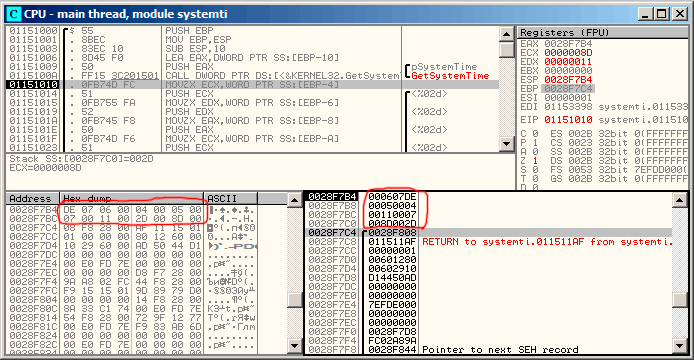
\includegraphics[scale=\FigScale]{patterns/15_structs/1_systemtime/olly_systemtime1.png}
\caption{\olly: \TT{GetSystemTime()} just executed}
\label{fig:struct_olly_1}
\end{figure}

The system time of the function execution on my computer is 9 december 2014, 22:29:52:

\begin{figure}[H]
\centering
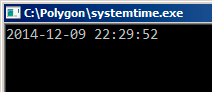
\includegraphics[scale=\NormalScale]{patterns/15_structs/1_systemtime/olly_systemtime2.png}
\caption{\olly: \printf output}
\label{fig:struct_olly_2}
\end{figure}

So we see these 16 bytes in the
data window: 
\begin{lstlisting}
DE 07 0C 00 02 00 09 00 16 00 1D 00 34 00 D4 03
\end{lstlisting}

Each two bytes represent one field of the structure. 
Since the \gls{endianness} is \IT{little endian}, 
we see the low byte first and then the high one.

Hence, these are the values currently stored in memory:

\begin{center}
\begin{tabular}{ | l | l | l | }
\hline
\headercolor{} Hexadecimal number & 
\headercolor{} decimal number & 
\headercolor{} field name \\
\hline
0x07DE & 2014	& wYear \\
\hline
0x000C & 12	& wMonth \\
\hline
0x0002 & 2	& wDayOfWeek \\
\hline
0x0009 & 9	& wDay \\
\hline
0x0016 & 22	& wHour \\
\hline
0x001D & 29	& wMinute \\
\hline
0x0034 & 52	& wSecond \\
\hline	
0x03D4 & 980	& wMilliseconds \\
\hline
\end{tabular}
\end{center}

The same values are seen in the stack window, but they are grouped as 32-bit values.

And then \printf just takes the values it needs and outputs them to the console.

Some values aren't output by \printf  (\TT{wDayOfWeek} and \TT{wMilliseconds}), 
but they are in memory right now, available for use.

